\chapter{Background Details}

\section{Automated Machine Learning}
Automated Machine Learning or AutoML, is the process of automating the time consuming task of Algorithm Selection and Optimizing the Hyper-Parameters. Traditional machine learning model creation is highly resource-intensive and requires significant domain knowledge and time to create and compare dozens of models. With AutoML, we will be able to accelerate the time it takes to get ML models with great ease and efficiency. There are many tools that offer to perform this complicated and time consuming task like Auto-Sklearn, Auto-Weka, Auto-Keras, etc. Apart from these tasks AutoML tools also perform feature selection, featuring engineering, data pre-processing and also analyse and tune the results. Among the various tasks performed by the AutoML Tools, the tasks that consume the most of the time are Algorithm Selection and Hpyer-Parameter Optimisation. 

\subsection{Algorithm Selection}
Algorithm Selection is usually done on an instance by instance basis, meaning different algorithm have to be chosen for different datasets. An algorithm which performs exceptionally well for one dataset may perform poorly for another. The task of choosing an algorithm is dependent on what data we have and how we choose to use it, meaning how the data is cleaned, encoded, imputed, distributed and also how they co-relate with other features or variables within the dataset. The manual task of algorithm selection involves studying and understanding the relationship between different features of the dataset, trying various types of pre-processing steps to bring out the inter-feature relationship which best explains the data. 

The tools which perform Algorithm Selection choose the best performing algorithm by predicting the performance of each algorithm for a given task by running various algorithms on a subset of the entire dataset repeatedly after performing different pre-processing steps and then choose the best performing algorithm on that subset for the task. Though this is just a over-simplified explanation of what the libraries do internally, this task is more of a straight forward approach which reduces the effort that a developer need to put in to select an algorithm. But this process comes with a huge trade-off, it takes up a lot of time, electricity and computational power before it could suggest the best suited algorithm for the task. Even if the task is to find the best algorithm for a previously seen dataset the entire process is repeated.

\subsection{Algorithm Configuration}

The task of Algorithm Configuration can be attributed to Hyper-Parameter Optimisation / Tuning, which is a process of selecting a set of optimal parameters for an algorithm for which it performs best on a dataset. A hyper-parameter is a parameter whose value is used control how a machine learning algorithm solves or learns to solve a given problem. Hyper-Parameter Optimisation of an Algorithm is a type of Optimisation problem. And a typical Optimisation problem consists of minimising or maximizing the set of parameters along with the metric. This task takes an expert with an in-depth domain knowledge a lot of time to solve, and is not something that can be performed with ease by a developer and hence the alternate approach of automating the task.

There are various optimisation strategies, among them the commonly used strategies are: Grid search, Random search, Hill Climbing and Bayesian optimization. The working of these strategies are out of scope of this paper, but the important thing to note is that these strategies takes up a great deal of time, electricity and computational power, before a optimal set of hyper-parameter can be chosen for an algorithm-dataset pair.

\section{Workflow of AutoML Libraries}
\label{workflow-automl}

In this section we will discuss about the workflow of AutoML libraries without getting to the details regarding the internal workings of the algorithms or the libraries. The figure \ref{automl-workflow-diagram} represents the workflow of a typical AutoML project for a given task or dataset. The data is split into training and testing datasets, the training dataset is first sent to the library for the purpose of model creation. Here, the dataset is pre-processed using various techniques like data-cleaning, data imputation, data encoding, feature selection, feature exploration, feature engineering, feature co-relation, etc..

\begin{figure}[t]
    \centering
    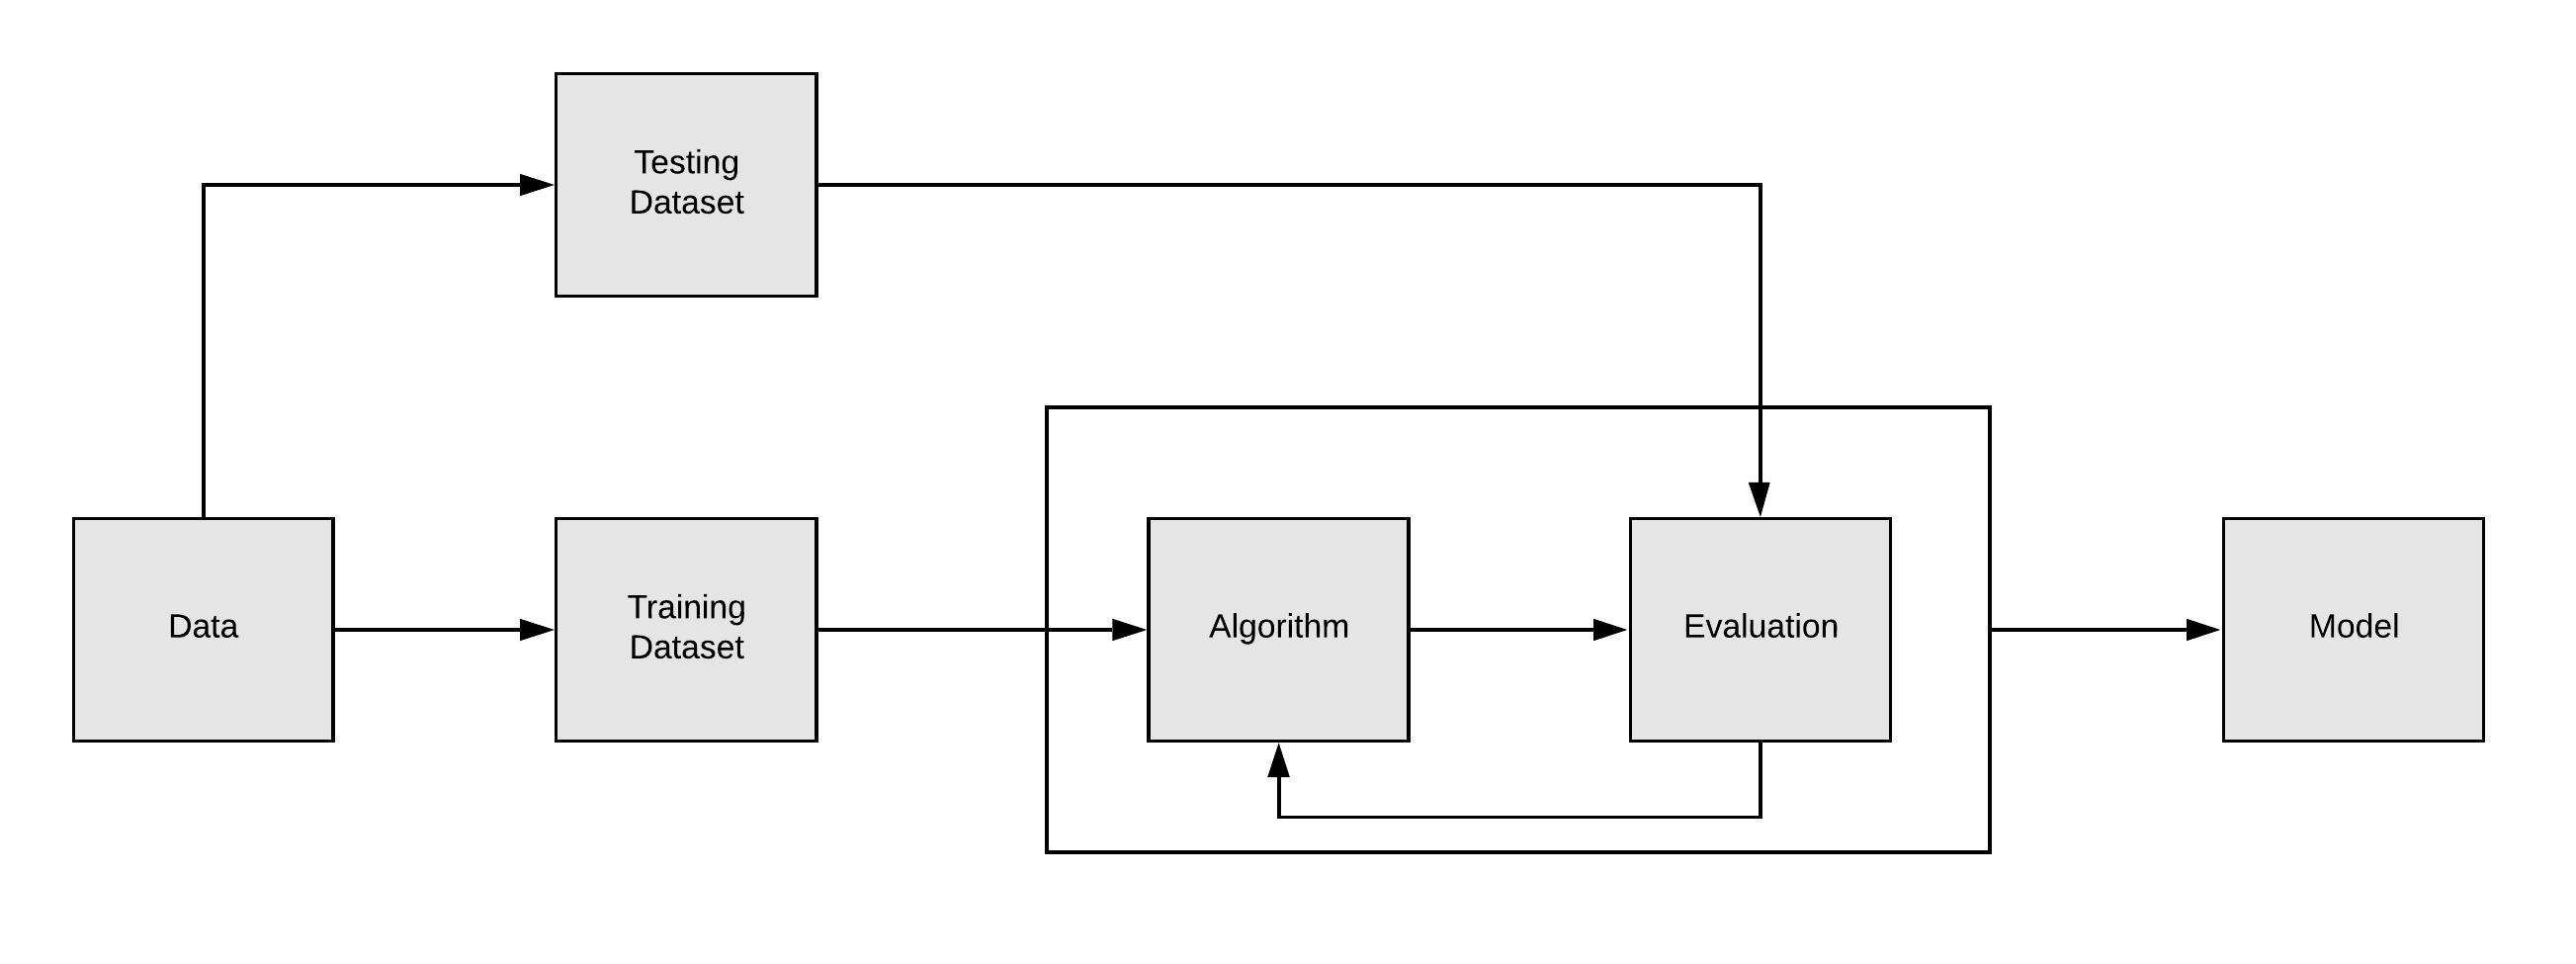
\includegraphics[width=16cm]{images/ML Workflow.jpeg}
    \caption{AutoML Workflow Diagram}
    \label{automl-workflow-diagram}
\end{figure}

Once, the data has been pre-processed, the dataset is split into a smaller subsets of the training dataset. One such subset is randomly chosen on which multiple algorithms are run to train and create a model for comparison and evaluation. Once the training and model creation of all chosen algorithms are completed, these models are evaluated based on multiple parameters one of which is their performance of an unseen data. When the performance metrics are calculated these models are evaluated and compared between each other and the best performing model is chosen for further training. Depending on the internal evaluation strategy of the AutoML tool used, more than one algorithm can be chosen for further training. Once these model(s) are chosen they are trained on various configurations of hyper-parameters using one of these search strategies; Grid Search, Randomized Search, Bayesian Optimization, etc. Once these models are trained and there hyper-parameters are optimised on the complete training dataset, they are evaluated against the testing dataset and the final best performing model is returned to the user.

%% a multi-line comment as an if statement
\if false

\section{Project Overview}
To tackle this repetitive and time consuming nature of these task, Dr. Joeran Beel proposed, what he called Federated Meta-Learning. Applying the concept of Federated Meta Learning, I have build an application called FMLearn to implement the same. Before explaining what the application is and what is does, some important information of this application are as follows. FMLearn is an application developed using the client-server model, which allows the exchange of meta-data about machine learning models and data for the purpose of meta-learned algorithm selection and configuration. In this Client-Server architecture the Client here is a popular Machine Learning package called Scikit-Learn which has been modified to the needs of the project. The client also enlists the help of another popular AutoML package for meta-data collection called Auto-Sklearn. 

\subsection{The Client: Scikit-Learn}
The client performs 2 crucial roles, one is to publish / send data to the server, which is then used by FMLearn to learn from and use this knowledge to make future predictions for tasks. The other task is to retrieve data from FMLearn, the data consists of Algorithm Predictions for previously seen or unseen datasets. The ideal choice for a client in such a role would be any popular and easy to use Machine Learning Library, and my choice was to use Scikit-Learn.

Scikit-learn \citep{scikit-learn} is a widely used, free and open source machine learning library\footnote{https://pypi.org/project/scikit-learn/}. I have used this as the client in the client-server model of my project to collect the information regarding how different classification, regression and clustering algorithms perform on various datasets and then publish / send this information about the model and other meta-data collected to the server - FMLearn - via the API endpoints which are made publicly available. It  also performs the role of retrieving the predicted algorithm for a previously seen or unseen task from the server via other exposed API's.

\subsection{The Server: FMLearn}
The server is a Python Application, which serves API's requests providing the caller with the requested details. It also acts as a knowledge base for all the data that is collected using the client, and learns from this knowledge base and suggests algorithms for a given task. It also has a very minimal user interface which explains the applications and provides links to various other useful information which might be required for the user.

\subsection{Meta-Features from Auto-Sklearn}
The tasks or datasets on which these algorithms run on are described by their meta-features which are obtained using the Auto-sklearn \citep{feurer:m} library via the client and this information about the meta-data about the data along with performance details of the algorithm on a particular task is sent / published to the server via an API call.

\fi

\section{Related Work}

%% a multi-line comment as an if statement
\if false

\section{Related Research}

\subsection{Paper1}
\subsection{Paper2}
\subsection{Paper3}
\subsection{Technology1}
\subsection{Technology2}

\section{Technology Used}
\subsection{why this stack}
\subsection{why client-server model}
\subsection{why scikit learn}

\fi


